\documentclass{article}
\usepackage{amsmath, amssymb, amsthm, mathtools}
\usepackage{enumitem}
\usepackage{tikz}
\usetikzlibrary{calc}
\usepackage[margin=1in]{geometry}

\tikzset{%
	add/.style args={#1 and #2}{to path={%
	($(\tikztostart)!-#1!(\tikztotarget)$)--($(\tikztotarget)!-#2!(\tikztostart)$)%
	\tikztonodes}}
} 

\title{Combinatorics: Homework 4}
\author{Jack Shi - A92122910}
\date{February 9, 2018}

\begin{document}
\maketitle

\begin{enumerate} [label=\textbf{\arabic*}.]
	% Problem 1
	\item Let $\mathcal{P}$ be a point configuration in $\mathbb{R}^3$. Let
		$\mathcal{L}$ denote the corresponding line configuration. Show that either
		$\mathcal{L}$ consists of a single line, or it contains an ordinary line
		(Hint: reduce to the two-dimensional case).\\
	
		Sylvester-Gallai Theorem:
		\begin{proof}
			Consider $\mathcal{S} = \{(L,P)\mid L\in\mathcal{L},\ P\in\mathcal{P},\
			P\not\in L$. This contains all pairs of line and point such that the point
			P is not on the line L.
			\paragraph{$\mathcal{S}=\emptyset$: } There does not exist a pair of point and line
			such that the point is not on the line. This means that all the points in
			$\mathcal{P}$ are colinear. $\mathcal{L}=\{L\}$, such that L contains all
			points in $\mathcal{P}$.
			\paragraph{$\mathcal{S}$ is non-empty: } Construct the following function:
			\begin{align*}
				d:f &\mapsto R_{>0}\\
				d(L,P) &= distance(P,L)
			\end{align*}
			Let $(L_0,P_0) = \underset{(L,P)}{argmin}\ distance(P,L)$:
				$$d(L_0,P_0)=min\{d(L,P)\mid (L,P) \in \mathcal{S}\}$$
			\subparagraph{Claim: } $L_0$ is an ordinary line.
			Since $L_0 \in \mathcal{L}$ it passes through two points $P_1,P_2 \in
			\mathcal{P}$. Since we can define a plane with any three points, let the
			following diagram be a plane in $\mathbb{R}^3$ that contains $P_0$, $P_1$,
			$P_3$:

			\begin{tikzpicture}[dot/.style={circle,inner sep=1pt,fill,name=#1}]
				\node [label={below:$L_0$}] at (-1.2, 0.8) {};
				\node [dot=A, label={below:$P_1$}] at (0, 0) {};
				\node [dot=B, label={below:$P_2$}] at (3, -1) {};
				\node [dot=C, label={right:$P_0$}] at (2, 0.5) {};
				\node [dot=D, label={below:$D$}] at ($(A)!(C)!(B)$) {};
				\draw [dashed] (D) -- (C);
				\draw [add=0.3 and 0.3](A) to (B);
			\end{tikzpicture}\\
			Let $\overline{P_0 D}$ is the shortest distance between $P_0$ and $D$.
			Assume towards a contrary that $L_0$ contains a third point $P_3$. Since
			this is now compressed to a plane, the line $L_1$ and point $P_3$ can be
			draw as follows:

			\subparagraph{Case 1: }$P_3$ is between D and $P_1$

			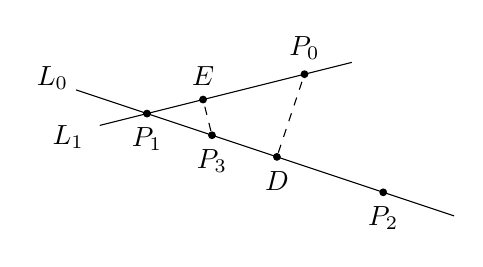
\begin{tikzpicture}[dot/.style={circle,inner sep=1pt,fill,name=#1}]
				\node [label={below:$L_0$}] at (-1.2, 0.85) {};
				\node [label={below:$L_1$}] at (-1, 0.1) {};
				\node [dot=A, label={below:$P_1$}] at (0, 0) {};
				\node [dot=B, label={below:$P_2$}] at (3, -1) {};
				\node [dot=C, label={above:$P_0$}] at (2, 0.5) {};
				\node [dot=D, label={below:$D$}] at ($(A)!(C)!(B)$) {};
				\node [dot=F, label={below:$P_3$}] at ($(A)!0.5!(D)$) {};
				\node [dot=E, label={above:$E$}] at ($(A)!(F)!(C)$) {};
				\draw [dashed] (D) -- (C);
				\draw [dashed] (F) -- (E);
				\draw [add=0.3 and 0.3](A) to (B);
				\draw [add=0.3 and 0.3](C) to (A);
			\end{tikzpicture}\\
			
			\subparagraph{Case 2: }$P_3$ is between D and $P_2$

			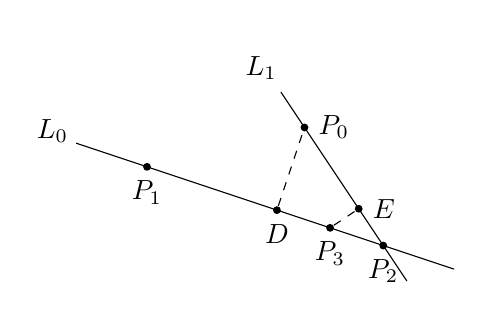
\begin{tikzpicture}[dot/.style={circle,inner sep=1pt,fill,name=#1}]
				\node [label={below:$L_0$}] at (-1.2, 0.85) {};
				\node [label={below:$L_1$}] at (1.45, 1.65) {};
				\node [dot=A, label={below:$P_1$}] at (0, 0) {};
				\node [dot=B, label={below:$P_2$}] at (3, -1) {};
				\node [dot=C, label={right:$P_0$}] at (2, 0.5) {};
				\node [dot=D, label={below:$D$}] at ($(A)!(C)!(B)$) {};
				\node [dot=F, label={below:$P_3$}] at ($(B)!0.5!(D)$) {};
				\node [dot=E, label={right:$E$}] at ($(B)!(F)!(C)$) {};
				\draw [dashed] (D) -- (C);
				\draw [dashed] (F) -- (E);
				\draw [add=0.3 and 0.3](A) to (B);
				\draw [add=0.3 and 0.3](C) to (B);
			\end{tikzpicture}\\

			Hence shown $\mathcal{S}$ a non-empty,  set. Any minimizer $(L_0,
			P_0)=\underset{(L,P)}{argmin}\ distance(P,L)$ result in a line $L_0$ that
			pass through exactly two points within $\mathcal{P}$
			
		\end{proof}

	% Problem 2
	\item A singel line drawn in the plane divides the plane into two regions. Two
		lines divide the pane into four regions, provided they are not parallel.
		\begin{enumerate} [label=\textbf{\alph*}.]
			% Problem 2a
			\item Determine the maximum number of regions into which three lines can
				divide the plane.

				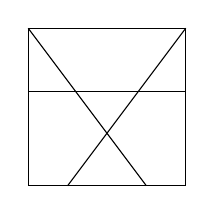
\begin{tikzpicture}\\
					\draw	(0, 0) -- (2, 0) -- (2, -2) -- (0, -2) -- (0, 0);
					\draw (0, 0) -- (1.5, -2);
					\draw (2, 0) -- (0.5, -2);
					\draw (0, -0.8) -- (2, -0.8);
				\end{tikzpicture}\\
				3 lines can divide the plane into a maximum of 7 regions.

			% Problem 2b
			\item Find a formula for the maximum number of regions into which n lines
				can divide the plane. Proove the correctness of the formula.
					\begin{align*}
					R(3) &= 7\\
					R(n) &= R(n-1) + n \qquad \forall n > 3
					\end{align*}
				This is because to maximize the number of regions generated by a new
				line, the new line should intersect with all old lines and also form a
				region by including the new line itself. This means the new line should
				add $(n-1) + 1$ regions on top of previous ones. The closed form of this
				formula is as follows:
					$$R(n) = 1 + \frac{n(n+1)}{2}$$

				\begin{proof} Show that the algorithm $R(n) = 1 + \frac{n(n+1)}{2}$ is
					correct by induction:
					\paragraph{Base Case: }
						\begin{align*}
						R(3) &= 1 + \frac{3(3+1)}{2}\\
						     &= 1 + 6\\
						     &=7
						\end{align*}

					\paragraph{Induction Hypothesis: }$R(n) = R(n-1) + n = 1 + \frac{n(n+1)}{2}$ yields
					the maximum numbers of regions that a plane can be divided into by n
					lines.

					\paragraph{Induction Step: }Wants to show $R(n+1)$ holds:
						\begin{align*}
							R(n+1) &= 1 + \frac{(n+1)(n+2)}{2}\\
							       &= 1 + \frac{n^2+3n+2}{2}\\
							       &= 1 + \frac{n^2+n+2n+2}{2}\\
							       &= \left(1 + \frac{n^2+n}{2}\right) + \left(\frac{2n}{2} +
										 \frac{2}{2}\right)\\
							       &= \left(1 + \frac{n(n+1)}{2} \right) + (n + 1)\\
										 &= R(n) + (n + 1)
						\end{align*}
					By the recursive definition $R(n) = R(n-1) + n$, $R$ holds for $n+1$,
					therefore $R(n)$ yields the maximum number of regions that a plane can
					be divided into by n lines.
				\end{proof}
		\end{enumerate}
\end{enumerate}

\end{document}

